% Лабораторная работа №2. Анализ и подготовка структур BCR::ABL1 WT и T315I
% Компиляция: pdflatex report.tex  (дважды, из папки report)
\documentclass[12pt,a4paper]{article}

\usepackage{cmap}
\usepackage[T2A]{fontenc}
\usepackage[utf8]{inputenc}
\usepackage[russian]{babel}
\usepackage[left=2.5cm,right=1.5cm,top=2cm,bottom=2cm]{geometry}
\usepackage{booktabs}
\usepackage{longtable}
\usepackage{array}
\usepackage{graphicx}
\usepackage{enumitem}
\usepackage{amsmath}
\usepackage{float}
\usepackage{caption}
\usepackage[hidelinks]{hyperref}
\usepackage[expansion=false]{microtype}

\captionsetup{font=small,labelfont=bf}
\setlength{\parindent}{1.25em}
\setlength{\emergencystretch}{3em}
\renewcommand{\arraystretch}{1.2}

\newcolumntype{L}[1]{>{\raggedright\arraybackslash}p{#1}}
\newcommand{\code}[1]{{\ttfamily #1}}

\title{\textbf{Лабораторная работа №2}\\[4pt]
Анализ и подготовка экспериментальных структур\\[4pt]
\large Объект исследования: BCR::ABL1 тирозинкиназа --- WT (2HYY) и T315I (3QRJ)}
\author{Шпока Владислав, Пясецкий Кирилл\\4 курс, 3 группа}
\date{4 октября 2026 г.}

\begin{document}
\maketitle

\section*{Цель работы}
Изучить две экспериментальные структуры киназного домена ABL1 --- нативную (WT) и
несущую мутацию T315I, --- оценить их качество и полноту, подготовить из них рабочие
файлы для последующего докинга и выполнить пространственное сравнение двух форм белка.

\section*{Исходные данные из лабораторной работы №1}

Работа продолжает лабораторную №1 и использует её результаты напрямую:

\begin{center}
\begin{tabular}{L{5.3cm}L{9.2cm}}
\toprule
\textbf{Результат работы №1} & \textbf{Как используется здесь} \\
\midrule
Мишень: ABL1, UniProt \code{P00519}, 1130 а.о. & Эталон нумерации остатков и
последовательности; файл \code{lab1/data/uniprot\_P00519.json} читается скриптом
подготовки \\
Киназный домен 242--493 & Границы области, внутри которой проверяются пропуски и
считается локальное RMSD \\
Gatekeeper Thr315 & Остаток, вокруг которого строится весь анализ \\
Выбранная структура WT: \textbf{2HYY} (2.40~\AA, лиганд STI --- иматиниб) &
Становится \code{WT\_original.cif} \\
Выбранная структура T315I: \textbf{3QRJ} (1.82~\AA, лиганд 919 --- ребастиниб) &
Становится \code{T315I\_original.cif} \\
Сайт связывания ATP: 248--256, 271, 316--322 & Проверка того, что пропуски не
задевают карман связывания \\
Петля активации 381--405 & Интерпретация участков наибольшего расхождения структур \\
\bottomrule
\end{tabular}
\end{center}

\section*{Замечание об инструментах}
Задание сформулировано в терминах UCSF ChimeraX. На рабочей машине ChimeraX не
установлен (в дистрибутивах PyPI его нет --- это отдельное настольное приложение
со своим интерпретатором), поэтому все операции выполнены программно через библиотеку
\code{gemmi} в скриптах \code{scripts/}. Для каждого пункта в отчёте приведена
\emph{эквивалентная последовательность команд ChimeraX}, дающая тот же результат, так
что работу можно повторить в графической программе без изменений. Все числа в отчёте
получены из реальных координат скачанных структур, иллюстрации построены по тем же
координатам.

\section{Подготовка исходных структур}

Структуры загружены с RCSB PDB в формате mmCIF
(\url{https://files.rcsb.org/download/2HYY.cif}, аналогично для 3QRJ) и сохранены как
\code{WT\_original.cif} и \code{T315I\_original.cif}.

\begin{center}
\begin{tabular}{L{4.4cm}L{5.1cm}L{5.1cm}}
\toprule
\textbf{Проверяемый пункт} & \textbf{WT} & \textbf{T315I} \\
\midrule
PDB ID & 2HYY & 3QRJ \\
Название белка & Human Abl kinase domain in complex with imatinib (STI571, Glivec) &
The crystal structure of human abl1 kinase domain T315I mutant in complex with DCC-2036 \\
Киназный домен присутствует? & да, остатки 235--498 перекрывают домен 242--493 &
да, остатки 234--496 перекрывают домен 242--493 \\
Мутации & нет (нативная последовательность) & только T315I \\
Метод & X-ray diffraction & X-ray diffraction \\
Разрешение & 2.40~\AA & 1.82~\AA \\
Ингибитор & есть: STI (иматиниб) & есть: 919 (ребастиниб, DCC-2036) \\
\bottomrule
\end{tabular}
\end{center}

\section{Текстовая структура PDB-файла}

В сохранённом файле \code{WT\_complex.pdb} координаты записаны строками \code{ATOM}
(атомы белка) и \code{HETATM} (всё, что не входит в полимер: лиганд, ионы, вода).
Пример первой строки файла:

\begin{verbatim}
ATOM      1  N   TRP A 235       2.281   3.258  18.672  1.00 89.25           N
|----| |---| |-| |-| | |--|      |-----| |-----| |----| |--| |---|           |
  1      2    3   4  5  6           7       8      9     10   11            12
\end{verbatim}

\begin{center}
\begin{tabular}{L{0.8cm}L{3.0cm}L{3.0cm}L{7.2cm}}
\toprule
\textbf{№} & \textbf{Колонки} & \textbf{Поле} & \textbf{Значение в примере} \\
\midrule
1 & 1--6 & тип записи & \code{ATOM} --- атом полимера \\
2 & 7--11 & серийный номер атома & 1 \\
3 & 13--16 & имя атома & \code{N} --- азот основной цепи \\
4 & 18--20 & имя остатка & \code{TRP} --- триптофан \\
5 & 22 & идентификатор цепи & \code{A} \\
6 & 23--26 & номер остатка & 235 \\
7--9 & 31--54 & координаты X, Y, Z & 2.281; 3.258; 18.672 (в ангстремах) \\
10 & 55--60 & заселённость (occupancy) & 1.00 \\
11 & 61--66 & B-фактор & 89.25 (высокий: N-конец подвижен) \\
12 & 77--78 & химический элемент & \code{N} \\
\bottomrule
\end{tabular}
\end{center}

\noindent Строка \code{HETATM 2075  C1  STI A 600 \ldots} устроена так же, но относится
к атому \code{C1} молекулы иматиниба (\code{STI}), которой присвоен номер 600 в цепи
\code{A}: лиганд нумеруется отдельно от белковой последовательности, что позволяет
выбирать его как самостоятельный объект.

\section{Открытие структуры}

\begin{verbatim}
open WT_original.cif
info #1
\end{verbatim}

\noindent Обе структуры открываются как модель \code{\#1}. Содержимое моделей:

\begin{center}
\begin{tabular}{L{3.4cm}L{5.4cm}L{5.4cm}}
\toprule
\textbf{Параметр} & \textbf{WT (2HYY)} & \textbf{T315I (3QRJ)} \\
\midrule
Номер модели & \#1 & \#1 (при повторном открытии --- \#2) \\
Цепей в модели & 4: A, B, C, D & 2: A, B \\
Полимерных сущностей & 1 (все цепи --- один и тот же белок) & 1 \\
Непополимерные компоненты & STI (4 копии), вода & 919 (2 копии), вода \\
\bottomrule
\end{tabular}
\end{center}

\noindent Наличие нескольких цепей --- следствие кристаллической упаковки
(несколько молекул в асимметричной ячейке), а не биологической олигомеризации
киназного домена. Для работы достаточно одной цепи.

\section{Определение белковой цепи}

По разделу \emph{Sequence} на странице RCSB обе цепи ссылаются на одну и ту же запись
UniProt \code{P00519} (результат лабораторной №1). Для дальнейшей работы выбрана
цепь~\code{A} в обеих структурах.

\begin{center}
\begin{tabular}{L{4.6cm}L{5.0cm}L{5.0cm}}
\toprule
\textbf{Параметр} & \textbf{WT (2HYY)} & \textbf{T315I (3QRJ)} \\
\midrule
PDB ID & 2HYY & 3QRJ \\
Номер модели & \#1 & \#1 \\
Ссылка на UniProt & P00519 (ABL1\_HUMAN) & P00519 (ABL1\_HUMAN) \\
Идентификатор цепи ABL1 & A & A \\
Разрешено остатков в цепи & 263 & 258 \\
Диапазон разрешённых остатков & 235--498 & 234--496 \\
Диапазон киназного домена & 242--493 (целиком внутри) & 242--493 (целиком внутри) \\
\bottomrule
\end{tabular}
\end{center}

\section{Ленточная модель}

\begin{verbatim}
cartoon #1/A
hide #1/A atoms
\end{verbatim}

\begin{figure}[H]
\centering
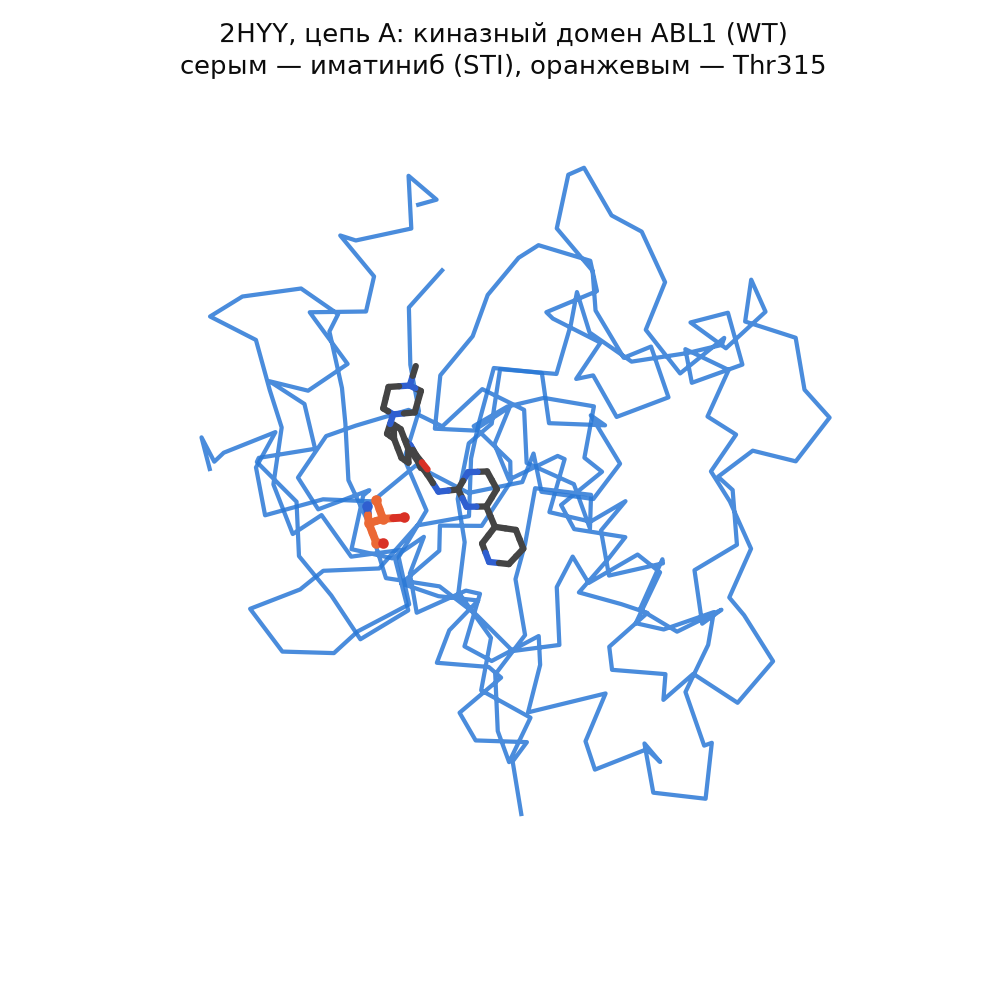
\includegraphics[width=0.78\linewidth]{../figures/fig_wt_fold.png}
\caption{Ход основной цепи киназного домена ABL1 (2HYY, цепь A), построенный по
координатам C$\alpha$. Видна характерная двухдольная архитектура протеинкиназы:
меньшая N-доля ($\beta$-слой) сверху, большая $\alpha$-спиральная C-доля снизу,
между ними --- щель, в которой лежит иматиниб (серым). Оранжевым показан
gatekeeper-остаток Thr315 на границе щели.}
\end{figure}

\section{Поиск позиции мутации}

\begin{verbatim}
select #1/A:315
show sel atoms
style sel stick
\end{verbatim}

\noindent Остаток с номером 315 найден в обеих структурах: в 2HYY это \textbf{THR}
(треонин), в 3QRJ --- \textbf{ILE} (изолейцин). То есть различие, ради которого
выбирались структуры, действительно присутствует в координатах, а не только в
аннотации записи.

\section{Проверка соответствия нумерации}

Нумерация проверена не на глаз, а сопоставлением: для каждого сдвига от $-40$ до $+40$
подсчитана доля остатков структуры, совпадающих с последовательностью UniProt
\code{P00519} в позиции \code{номер\_в\_PDB} $+$ \code{сдвиг}.

\begin{center}
\begin{tabular}{L{5.0cm}L{4.8cm}L{4.8cm}}
\toprule
\textbf{Параметр} & \textbf{WT (2HYY)} & \textbf{T315I (3QRJ)} \\
\midrule
Позиция в UniProt & 315 & 315 \\
Номер остатка в структуре & 315 & 315 \\
Найденный сдвиг нумерации & $0$ & $0$ \\
Доля совпадений при этом сдвиге & 100{,}0\,\% (263 из 263) & 99{,}6\,\% (257 из 258) \\
Совпадает ли нумерация? & да, полностью & да \\
\bottomrule
\end{tabular}
\end{center}

\noindent Обе структуры используют нумерацию изоформы 1a, ту же, что и UniProt, поэтому
никакого пересчёта не требуется. Единственное несовпадение в 3QRJ --- это и есть остаток
315 (в UniProt \code{T}, в структуре \code{I}): алгоритм сравнивает последовательности,
и мутация честно проявляется как одно расхождение. Это косвенная проверка того, что
мутация в структуре ровно одна. Отдельно отметим, что в части публикаций и записей
используется нумерация изоформы 1b, где тот же остаток --- Thr334; к выбранным
структурам это не относится.

\section{Полнота структуры: отсутствующие участки}

\begin{center}
\begin{tabular}{L{4.8cm}L{4.9cm}L{4.9cm}}
\toprule
\textbf{Параметр} & \textbf{WT (2HYY), цепь A} & \textbf{T315I (3QRJ), цепь A} \\
\midrule
Диапазон разрешённых остатков & 235--498 & 234--496 \\
Внутренние пропуски & 275 (1 остаток) & 274--278 (5 остатков) \\
Пропуски внутри киназного домена 242--493 & да, 275 & да, 274--278 \\
Задевают ли пропуски позицию 315? & нет & нет \\
Задевают ли пропуски сайт связывания? & нет & нет \\
Остатков сайта связывания разрешено & 25 из 25 & 27 из 27 \\
\bottomrule
\end{tabular}
\end{center}

\noindent\textbf{Вывод о влиянии на дальнейший анализ.} Пропуски есть в обеих
структурах, но лежат в петле между $\beta$3 и $\alpha$C (участок 274--278), которая
выходит на поверхность белка и не формирует карман связывания. Ни один из остатков,
контактирующих с лигандом, не потерян: сайт связывания разрешён полностью в обеих
структурах. Поэтому для докинга и анализа взаимодействий структуры пригодны без
достройки недостающих петель. Достраивать участок 274--278 потребовалось бы только
при молекулярной динамике, где разрыв цепи недопустим.

\section{Сокристаллизованный ингибитор}

\begin{verbatim}
select #1:STI
show sel atoms
style sel stick
\end{verbatim}

\begin{center}
\begin{tabular}{L{4.4cm}L{5.1cm}L{5.1cm}}
\toprule
\textbf{Параметр} & \textbf{WT (2HYY)} & \textbf{T315I (3QRJ)} \\
\midrule
Название ингибитора & иматиниб (STI571, Gleevec) & ребастиниб (DCC-2036) \\
Код химического компонента & \code{STI} & \code{919} \\
Копий в структуре & 4 (по одной на цепь) & 2 (по одной на цепь) \\
Исследуемая цепь & A & A \\
Атомов в молекуле (без H) & 37 & 41 \\
Остатков белка в контакте ($\le 4{,}5$~\AA) & 25 & 27 \\
Положение остатка 315 относительно лиганда & непосредственно в кармане, контакт есть &
непосредственно в кармане, контакт есть \\
\bottomrule
\end{tabular}
\end{center}

\noindent Остатки сайта связывания (в радиусе 4{,}5~\AA{} от лиганда) для 2HYY:
Leu248, Tyr253, Val256, Ala269, Val270, Lys271, Glu286, Val289, Met290, Ile293, Val299,
Ile313, \textbf{Thr315}, Glu316, Phe317, Met318, Gly321, Phe359, Ile360, His361, Arg362,
Leu370, Ala380, Asp381, Phe382. Для 3QRJ: Leu248, Val256, Ala269, Lys271, Glu282,
Glu286, Val289, Met290, Ile293, Leu298, Val299, Ile313, \textbf{Ile315}, Glu316, Phe317,
Met318, Thr319, Gly321, Leu354, Phe359, His361, Leu370, Val379, Ala380, Asp381, Phe382,
Gly383.

\medskip
\noindent Существенно, что остаток 315 входит в список контактов в обеих структурах ---
то есть gatekeeper не просто «рядом», а непосредственно образует стенку кармана. В обоих
списках присутствует мотив DFG (Asp381--Phe382--Gly383) и каталитический Lys271, что
подтверждает: лиганд занимает именно ATP-карман.

\begin{figure}[H]
\centering
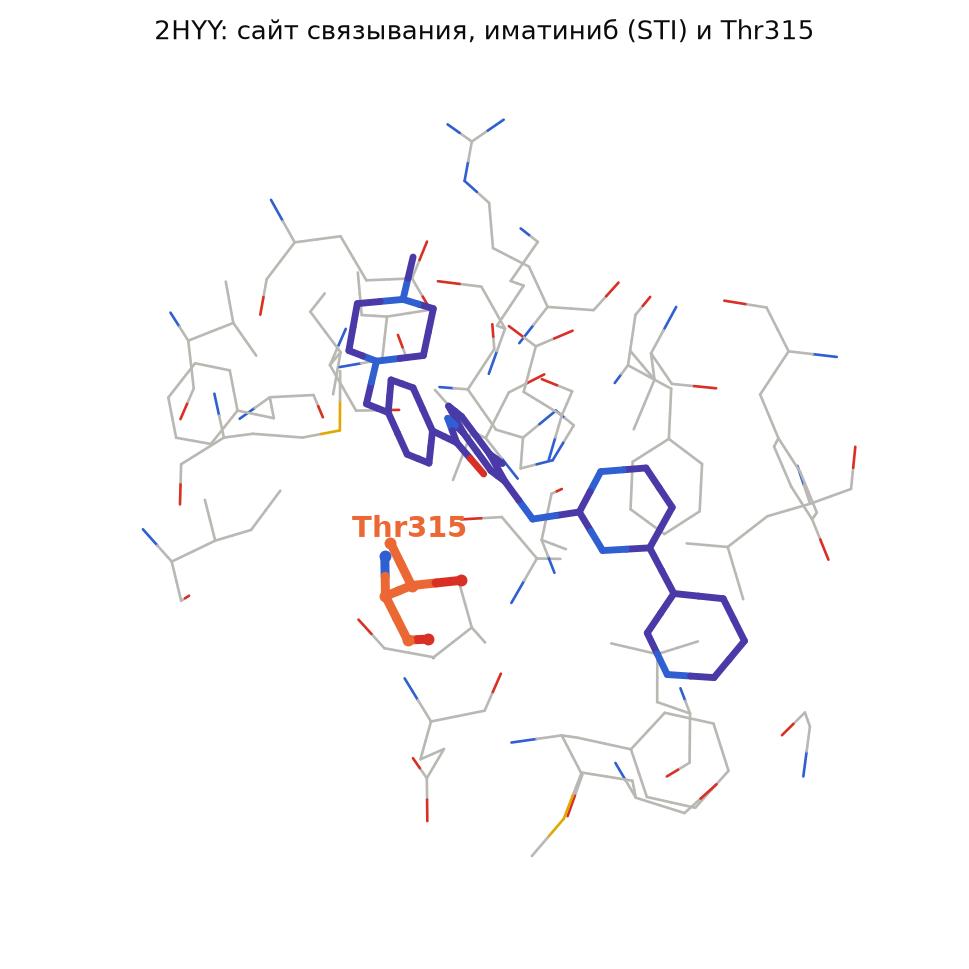
\includegraphics[width=0.73\linewidth]{../figures/fig_site_wt.png}
\caption{Сайт связывания 2HYY: иматиниб (фиолетовым) и Thr315 (оранжевым) в окружении
25 контактирующих остатков (тонкими линиями). Атомы окрашены по элементам: азот ---
синий, кислород --- красный, сера --- жёлтая.}
\end{figure}

\begin{figure}[H]
\centering
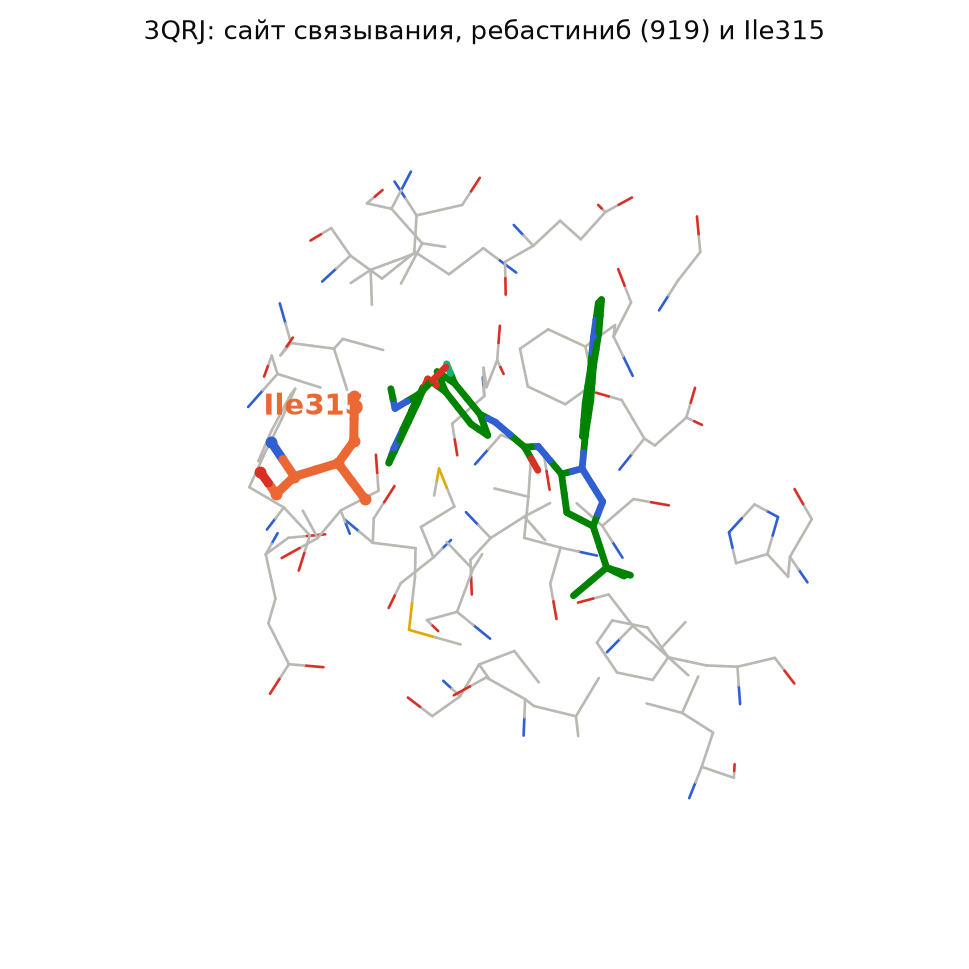
\includegraphics[width=0.73\linewidth]{../figures/fig_site_t315i.png}
\caption{Сайт связывания 3QRJ: ребастиниб (зелёным) и Ile315 (оранжевым). Разветвлённая
боковая цепь изолейцина занимает заметно больший объём, чем гидроксильная группа
треонина на предыдущем рисунке.}
\end{figure}

\section{Дополнительные компоненты структуры}

\begin{verbatim}
select solvent
select ligand
\end{verbatim}

\begin{center}
\begin{tabular}{L{4.6cm}L{5.0cm}L{5.0cm}}
\toprule
\textbf{Компонент} & \textbf{WT (2HYY)} & \textbf{T315I (3QRJ)} \\
\midrule
Вода (\code{HOH}) во всей модели & 200 молекул & 243 молекулы \\
Вода в цепи A & 51 молекула & 127 молекул \\
Ионы металлов & нет & нет \\
Криопротекторы, буферные добавки & нет & нет \\
Лиганд-ингибитор & \code{STI}, 4 копии & \code{919}, 2 копии \\
\bottomrule
\end{tabular}
\end{center}

\noindent Структуры «чистые»: кроме белка, ингибитора и воды, в них ничего нет. Воды
в 3QRJ заметно больше при меньшем числе цепей --- прямое следствие лучшего разрешения
(1{,}82~\AA{} против 2{,}40~\AA): при более высоком разрешении различимо больше
упорядоченных молекул растворителя. Вода и прочий растворитель в рабочие файлы не
включались: для докинга поверхность кармана обычно готовят без кристаллографической
воды.

\section{Файл «белок + ингибитор»}

\begin{verbatim}
select clear
select (#1/A & protein) | (#1:STI)
save WT_complex.pdb models #1 selectedOnly true
\end{verbatim}

\begin{center}
\begin{tabular}{L{4.6cm}L{4.1cm}L{2.3cm}L{2.3cm}}
\toprule
\textbf{Файл} & \textbf{Содержимое} & \textbf{Остатков} & \textbf{Атомов} \\
\midrule
\code{WT\_complex.pdb} & цепь A 2HYY + иматиниб & 264 & 2110 \\
\code{T315I\_complex.pdb} & цепь A 3QRJ + ребастиниб & 259 & 2116 \\
\bottomrule
\end{tabular}
\end{center}

\section{Файл только белка}

\begin{verbatim}
select clear
select #1/A & protein
save WT_protein.pdb models #1 selectedOnly true
\end{verbatim}

\begin{center}
\begin{tabular}{L{4.6cm}L{4.1cm}L{2.3cm}L{2.3cm}}
\toprule
\textbf{Файл} & \textbf{Содержимое} & \textbf{Остатков} & \textbf{Атомов} \\
\midrule
\code{WT\_protein.pdb} & цепь A 2HYY, только белок & 263 & 2073 \\
\code{T315I\_protein.pdb} & цепь A 3QRJ, только белок & 258 & 2075 \\
\bottomrule
\end{tabular}
\end{center}

\noindent Разница между парами файлов --- ровно один остаток и 37 (соответственно 41)
атомов: это и есть молекула ингибитора. Таким образом, для каждой формы белка получено
по три файла: \code{*\_original.cif}, \code{*\_complex.pdb}, \code{*\_protein.pdb} ---
всего шесть. Файлы «комплекс» нужны для валидации протокола докинга редокингом
(лиганд с известной позой), файлы «только белок» --- как приёмник для докинга новых
соединений.

\section{Подготовка к сравнению}

\begin{verbatim}
close session
open WT_original.cif
open T315I_original.cif
\end{verbatim}

\noindent После повторного открытия 2HYY получает номер \code{\#1} (цепи A, B, C, D),
3QRJ --- номер \code{\#2} (цепи A, B). Сравниваются цепи \code{\#1/A} и \code{\#2/A}.

\section{Наложение структур}

\begin{verbatim}
matchmaker #2/A to #1/A pairing ss
\end{verbatim}

\noindent В скрипте \code{scripts/}\allowbreak\code{superpose.py} выполнена эквивалентная процедура.
Поскольку в разделе~7 показано, что нумерация обеих структур совпадает с UniProt
(сдвиг 0), пары остатков строились прямо по номерам --- это точнее, чем выравнивание
последовательностей. Далее применено совмещение методом Кабша и то же итеративное
отбрасывание (iterative pruning) пар, расходящихся больше чем на 2{,}0~\AA, которое по
умолчанию делает Matchmaker.

\section{Результаты наложения}

\begin{center}
\begin{tabular}{L{8.8cm}L{5.7cm}}
\toprule
\textbf{Показатель} & \textbf{Значение} \\
\midrule
Пар остатков до отбрасывания & 257 \\
RMSD по всем парам & \textbf{1{,}292~\AA} \\
Порог отбрасывания & 2{,}0~\AA \\
Итераций отбрасывания & 4 \\
Пар остатков после отбрасывания & 242 \\
RMSD после отбрасывания & \textbf{0{,}815~\AA} \\
RMSD внутри киназного домена (242--493) & 1{,}301~\AA{} (247 пар) \\
RMSD в окрестности остатка 315 ($\pm 5$) & 0{,}920~\AA{} (11 пар) \\
Отклонение C$\alpha$ самого остатка 315 & 0{,}386~\AA \\
\bottomrule
\end{tabular}
\end{center}

\begin{figure}[H]
\centering
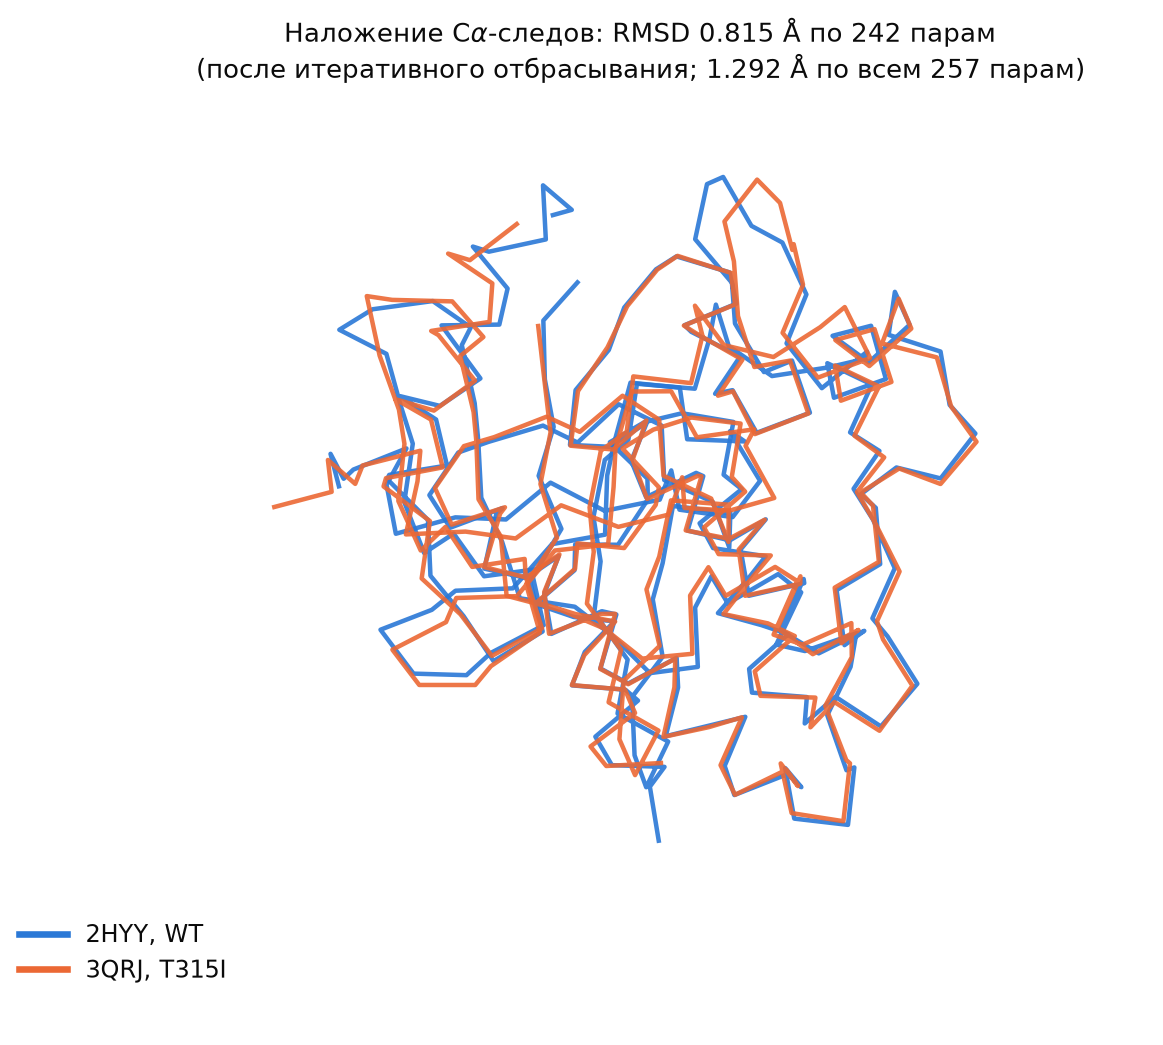
\includegraphics[width=0.8\linewidth]{../figures/fig_superposition.png}
\caption{Наложение C$\alpha$-следов 2HYY (WT, синий) и 3QRJ (T315I, оранжевый).
Общая укладка совпадает практически полностью.}
\end{figure}

\noindent Значение 0{,}815~\AA{} по 242 парам означает, что две структуры совпадают по
укладке в пределах экспериментальной точности: для кристаллических структур одного белка
с разрешением 1{,}8--2{,}4~\AA{} типичная «погрешность воспроизводимости» составляет
как раз несколько десятых ангстрема. Разница между 1{,}292~\AA{} по всем парам и
0{,}815~\AA{} после отбрасывания говорит, что расхождение создаётся не всей структурой,
а небольшим числом остатков: 15 отброшенных пар из 257.

\section{Локальное сравнение позиции мутации}

\begin{verbatim}
select #1/A:315 | #2/A:315
show sel atoms
style sel stick
\end{verbatim}

\begin{figure}[H]
\centering
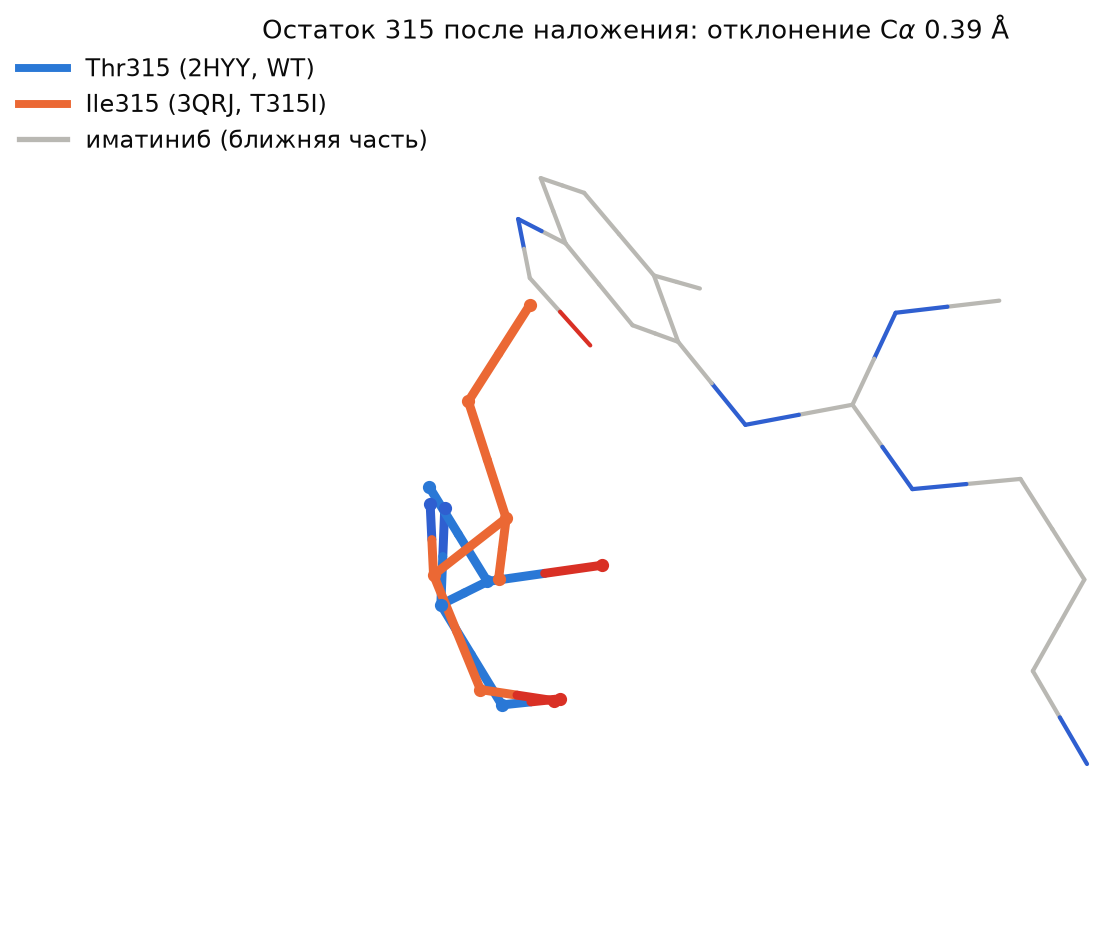
\includegraphics[width=0.78\linewidth]{../figures/fig_315_overlay.png}
\caption{Thr315 (синий) и Ile315 (оранжевый) после наложения. Основная цепь совпадает
(отклонение C$\alpha$ 0{,}386~\AA), но боковая цепь изолейцина разветвлена и уходит
заметно дальше в сторону кармана, где у WT располагается часть молекулы иматиниба
(серым).}
\end{figure}

\begin{figure}[H]
\centering
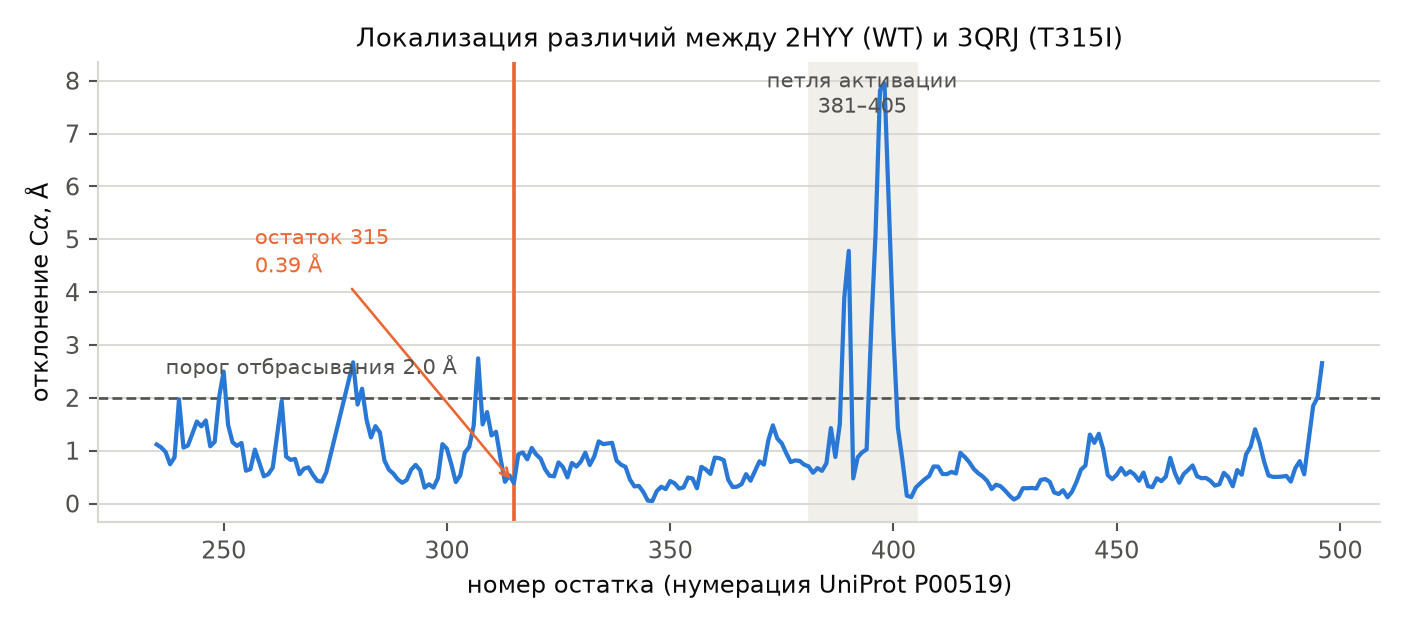
\includegraphics[width=\linewidth]{../figures/fig_deviation.png}
\caption{Отклонение C$\alpha$ по остаткам после наложения. Почти на всём протяжении
цепи оно меньше 1~\AA. Выброс до 8~\AA{} приходится на остатки 389--400 --- петлю
активации (381--405), выделенную серым. В позиции 315 (вертикальная оранжевая линия)
отклонение минимально.}
\end{figure}

\noindent\textbf{Насколько сходна общая структура?} Очень сходна: 0{,}815~\AA{} по 242
парам --- это уровень совпадения двух кристаллических форм одного и того же белка.
Замена Thr$\rightarrow$Ile не перестраивает укладку киназного домена.

\medskip
\noindent\textbf{Можно ли считать глобальное RMSD показателем полной идентичности
участка связывания?} Нет, и это главный методический вывод работы. Аргументы:

\begin{enumerate}[leftmargin=*,topsep=2pt,itemsep=3pt]
\item \textbf{Глобальное RMSD усредняет по сотням остатков.} 257 пар сглаживают любое
локальное различие: изменение в одном остатке даёт вклад порядка
$\sqrt{1/257} \approx 6\,\%$ и просто теряется в среднем.
\item \textbf{RMSD считается по C$\alpha$, а мутация меняет боковую цепь.} Отклонение
C$\alpha$ остатка 315 составляет 0{,}386~\AA{} --- меньше среднего по структуре. С точки
зрения основной цепи позиция 315 «не изменилась вообще», тогда как объём боковой цепи
вырос со $\approx$116 до $\approx$167~\AA$^3$, и именно это закрывает вход в
гидрофобный карман.
\item \textbf{Наибольшие расхождения лежат не там, где мутация.} Отброшенные пары
сосредоточены в остатках 389--400 (максимум 7{,}95~\AA{} на остатке 398) --- это петля
активации, подвижный элемент, конформация которого определяется связанным лигандом
(иматиниб и ребастиниб --- разные молекулы) и условиями кристаллизации, а не мутацией.
То есть крупнейшее различие между структурами к T315I прямого отношения не имеет.
\item \textbf{Следствие для дальнейшей работы.} Вывод «структуры почти одинаковы,
значит и карманы одинаковы» неверен. Сравнивать нужно локально: объём кармана, набор
контактов, наличие водородной связи с остатком 315. Это предмет следующей лабораторной
работы по межатомным взаимодействиям.
\end{enumerate}

\section{Паспорт структур}

\begin{center}
\begin{tabular}{L{4.8cm}L{4.9cm}L{4.9cm}}
\toprule
\textbf{Параметр} & \textbf{BCR::ABL1 WT} & \textbf{BCR::ABL1 T315I} \\
\midrule
PDB ID & 2HYY & 3QRJ \\
Экспериментальный метод & X-ray diffraction & X-ray diffraction \\
Пространственное разрешение & 2.40~\AA & 1.82~\AA \\
Исследуемая цепь & A & A \\
Диапазон киназного домена & 242--493 (в структуре 235--498) &
242--493 (в структуре 234--496) \\
Дополнительные мутации & нет & нет (только T315I) \\
Отсутствующие остатки & 275 (1 остаток) & 274--278 (5 остатков) \\
Пропуски в участке связывания & нет & нет \\
Сокристаллизованный ингибитор & иматиниб & ребастиниб (DCC-2036) \\
Код ингибитора & \code{STI} & \code{919} \\
Найден ли Thr315 / Ile315 & да, THR315 & да, ILE315 \\
Проверена ли нумерация по UniProt & да, сдвиг 0, совпадение 100\,\% &
да, сдвиг 0, совпадение 99{,}6\,\% \\
Пригодна ли для дальнейшего анализа & да & да \\
\bottomrule
\end{tabular}
\end{center}

\medskip
\noindent\textbf{Вывод о пригодности 2HYY.} Структура пригодна. Это человеческий ABL1
без посторонних мутаций, нумерация полностью совпадает с UniProt, сайт связывания
разрешён целиком, присутствует эталонный ингибитор 1-го поколения с известной позой.
Ограничение --- умеренное разрешение 2{,}40~\AA{} и единственный пропуск в поверхностной
петле, на карман не влияющий.

\medskip
\noindent\textbf{Вывод о пригодности 3QRJ.} Структура пригодна и по качеству данных даже
предпочтительнее: разрешение 1{,}82~\AA{} --- лучшее среди доступных T315I-структур.
Единственная замена в последовательности --- интересующая нас T315I, что подтверждено
сравнением с UniProt. Пропуск 274--278 длиннее, чем в 2HYY, но лежит в той же
поверхностной петле и сайта связывания не затрагивает.

\section{Состав сданных материалов}

\begin{center}
\begin{tabular}{L{6.0cm}L{8.5cm}}
\toprule
\textbf{Файл} & \textbf{Описание} \\
\midrule
\code{structures/}\allowbreak\code{WT\_original.cif} & 2HYY, исходная запись RCSB \\
\code{structures/}\allowbreak\code{T315I\_original.cif} & 3QRJ, исходная запись RCSB \\
\code{structures/}\allowbreak\code{WT\_complex.pdb} & цепь A + иматиниб (264 остатка, 2110 атомов) \\
\code{structures/}\allowbreak\code{T315I\_complex.pdb} & цепь A + ребастиниб (259 остатков, 2116 атомов) \\
\code{structures/}\allowbreak\code{WT\_protein.pdb} & цепь A, только белок (263 остатка, 2073 атома) \\
\code{structures/}\allowbreak\code{T315I\_protein.pdb} & цепь A, только белок (258 остатков, 2075 атомов) \\
\code{structures/}\allowbreak\code{T315I\_}\allowbreak\code{superposed\_}\allowbreak\code{on\_WT.pdb} & 3QRJ после совмещения с 2HYY \\
\code{figures/} & шесть иллюстраций, построенных по координатам \\
\code{scripts/}\allowbreak\code{prepare\_structures.py} & загрузка, анализ, сохранение рабочих файлов \\
\code{scripts/}\allowbreak\code{superpose.py} & наложение, RMSD, итеративное отбрасывание \\
\code{scripts/}\allowbreak\code{make\_figures.py} & построение иллюстраций \\
\code{data/analysis.json}, \code{data/superposition.json} & все числовые результаты \\
\code{report/report.pdf} & настоящий отчёт \\
\code{guide/guide.pdf} & подробный разбор теории и хода работы \\
\bottomrule
\end{tabular}
\end{center}

\medskip
\noindent\textbf{Прослеживаемость.} Цепочка преобразования полностью воспроизводима:
запись RCSB (\code{2HYY.cif}) $\rightarrow$ выбор цепи A и проверка нумерации по UniProt
$\rightarrow$ отделение белка и лиганда от воды $\rightarrow$ рабочие файлы
\code{WT\_complex.pdb} и \code{WT\_protein.pdb} $\rightarrow$ наложение с мутантной
формой. Каждый шаг выполняется скриптом, все промежуточные числа сохранены в
\code{data/*.json}.

\vspace{1cm}
\noindent Подписи студентов: \underline{\hspace{5cm}} \hfill Дата: \underline{\hspace{3.5cm}}

\end{document}
